%%
%% Draft article prepared with the Elsevier elsarticle class
%% for the journal Neurocomputing (Elsevier).
%% Each chapter lives in an independent file under ./sections/.
%% This draft is centered on the GT-conditioned CVAE algorithm.
%%
\documentclass[preprint,12pt]{elsarticle}

%% Useful packages
\usepackage[T1]{fontenc}
\usepackage{lmodern}
\usepackage{amssymb}
\usepackage{amsmath}
\usepackage{booktabs}
\usepackage{multirow}
\usepackage{algorithm}
\usepackage{algorithmic}
\usepackage{graphicx}
\usepackage{float}
\usepackage{xcolor}
\usepackage{tikz}
\usetikzlibrary{positioning, fit, calc}
\usepackage{listings}

%% Allow LaTeX to stretch lines slightly to avoid paragraph-level overfull
\setlength{\emergencystretch}{2em}

%% Listings style for the code snippets (appendix)
\lstset{
  basicstyle=\ttfamily\footnotesize,
  keywordstyle=\bfseries\color{blue!60!black},
  commentstyle=\color{green!45!black},
  stringstyle=\color{red!60!black},
  showstringspaces=false,
  numbers=left,
  numberstyle=\tiny\color{gray},
  frame=single,
  breaklines=true,
  captionpos=b,
  aboveskip=8pt,
  belowskip=6pt,
  xleftmargin=1.6em,
}

\journal{Neurocomputing}

\begin{document}

\begin{frontmatter}

%% Title, authors and addresses -----------------------------------------
\title{GT-Conditioned Variational Gaussian Splatting for Sparse-View
Cone-Beam CT Reconstruction}

%% Authors (to be completed before submission)
\author[aff1]{Author One\corref{cor1}}
\ead{author.one@example.edu}
\cortext[cor1]{Corresponding author}
\author[aff1]{Author Two}
\author[aff1]{Author Three}

\affiliation[aff1]{organization={Department of Biomedical Engineering, Example University},
            addressline={1 Example Road},
            city={City},
            postcode={000000},
            state={},
            country={Country}}

%%
%% Abstract / keywords are contained in abstract.tex (independent file).
%%
%% ============================================================================
%% Abstract and keywords (independent file, included inside \begin{frontmatter})
%% ============================================================================

\begin{abstract}
Sparse-view cone-beam CT (CBCT) reconstruction aims to recover a tomographic
volume from an extremely limited set of projection views, which is an
ill-posed inverse problem that traditional methods make it difficult to 
achieve effective reconstruction, and is typically solved with deterministic
deep networks. A probabilistic formulation can in principle quantify
reconstruction uncertainty and exploit privileged information --- dense views
or even the ground-truth volume --- during training, as long as inference
never depends on it. In this work we present the \emph{GT-conditioned CVAE}
 a conditional variational extension of the 3D-Gaussian-splatting CBCT
reconstructor. During training only, a lightweight 3D convolutional network
encodes the ground-truth volume into a 32-dimensional descriptor that
conditions the variational posterior $q(z\mid C,Y)$ over a 64-dimensional
global scene latent, while a sparse-view neural-process prior
$p(z\mid C)$ is trained jointly. At deployment the GT encoder and the
posterior are discarded: $z$ is drawn exclusively from the sparse-view prior,
so inference requires exactly the same inputs as the deterministic backbone
and additionally yields per-point predictive variance from $N{=}8$
Monte-Carlo samples. The decoder renders exclusively from the sparse
context features, so the latent is the sole channel of dense information
during training. On the LUNA16 CBCT benchmark with six
projections, the GT-conditioned CVAE reaches $29.50$\,dB PSNR /
$0.868$\,SSIM, within $0.04$\,dB of the deterministic backbone
($29.54$\,dB / $0.870$\,SSIM), while providing calibrated deployment-side
uncertainty estimates at no additional inference cost. Ablations
quantify the decisive design choices -- posterior access to the ground
truth and fusion token initialization -- for future probabilistic CBCT
models.
\end{abstract}

%% Research highlights
\begin{highlights}
\item A GT-conditioned CVAE for Gaussian-splatting sparse-view CBCT
reconstruction: ground truth is encoded into the variational posterior
during training only.
\item Deployment discards both the GT encoder and dense views, sampling
exclusively from a sparse-view prior; per-point predictive variance comes
for free from Monte-Carlo estimation.
\item Ablations isolate the decisive design choices: posterior access to
the ground truth and fusion token initialization ($\sim\!2$\,dB), with the
decoder routed through the context features.
\end{highlights}

%% Keywords
\begin{keyword}
Sparse-view CBCT reconstruction \sep 3D Gaussian splatting \sep
conditional variational autoencoder \sep variational inference \sep
latent neural processes \sep uncertainty estimation
\end{keyword}

\end{frontmatter}

%% Table of contents -----------------------------------------
%% Each numbered section below corresponds to one independent .tex file:
%%
%% Chapter 1: Introduction
%% Independent file, included by ../main.tex
%% This draft is centered on the GT-conditioned CVAE algorithm.
%%

\section{Introduction}
\label{sec:intro}

Cone-beam computed tomography (CBCT) is a cornerstone of image-guided
procedures in radiation therapy and interventional radiology, offering
volumetric imaging with compact gantry geometries. Clinical workflows,
however, place hard limits on the number of projection views that can be
acquired: fewer views reduce radiation dose and shorten scan times, but
dramatically undersample the Fourier domain of the object. Sparse-view CBCT
reconstruction -- recovery of a high-quality volume from a handful of
projections, typically far below the hundreds required by analytical
reconstruction -- is therefore an ill-posed inverse problem whose solution
requires strong prior knowledge of anatomy.

Deep learning has become the dominant tool for this task. Neural
reconstruction methods range from direct 2D$\to$3D back-projection networks
to score-based and diffusion models, and recent work has shown that
explicit scene representations such as 3D Gaussian splatting (3DGS)
\cite{kerbl2023gaussiansplats} provide an outstanding inductive bias for
tomographic volumes: compact, differentiable, and easily supervised by
projection consistency. The DIF-Gaussian framework \cite{lin2024difgaussian}
demonstrated that a splatting-based reconstructor can produce accurate
volumes from as few as six cone-beam projections.

Despite these advances, the vast majority of sparse-view CBCT models are
\emph{deterministic}: they map a fixed set of views to a single volume and
output no measure of confidence. This is unsatisfactory in a clinical
setting, where reconstruction noise and ambiguity are spatially
inhomogeneous and task-relevant, and where downstream planning decisions
(e.g., dose painting or target delineation) should ideally consume
calibrated uncertainty, not a point estimate.

A natural remedy is a \emph{conditional variational} formulation. During
training, privileged information that will not be available at deployment --
the dense-view set, or even the ground-truth volume itself -- can be
encoded into a variational posterior $q(z\mid C,Y)$ to concentrate the
latent code on target-specific content and tighten the evidence lower
bound. At deployment this posterior is discarded, and the reconstruction is
generated by sampling a sparse-view prior $p(z\mid C)$. If the training and
deployment information flows are carefully separated, such a design yields
both accuracy and per-point uncertainty from the very same model. If they
are not separated, a subtle and common failure appears: when the training
decoder can read dense-view features directly, the latent becomes redundant
and the variational posterior \emph{collapses} onto an uninformative prior,
silently degrading the deployment path.

In this paper we design, build, and rigorously evaluate a
\emph{GT-conditioned CVAE} on top of the Gaussian-splatting CBCT
reconstructor. Our contributions are:

\begin{enumerate}
\item \textbf{A conditional variational formulation for splatting-based
CBCT reconstruction.} We inject a tractable 64-dimensional global latent
variable into the Gaussian-splatting decoder through feature-wise linear
modulation (FiLM), with a neural-process prior $p(z\mid C)$ computed from
the sparse context views $C$ alone.

\item \textbf{The GT-conditioned CVAE.} During training only, a
lightweight 3D CNN ($1\to16\to16\to32$ channels) encodes the ground-truth
volume into a 32-dimensional descriptor that conditions the variational
posterior $q(z\mid C,Y)$; the objective simultaneously supervises the
deployment-side prior. At inference the GT encoder and posterior are
discarded and $z\sim p(z\mid C)$; \emph{no} ground truth or dense views are
required, and per-point predictive variance comes for free from $N{=}8$
Monte-Carlo sampling.

\item \textbf{Empirical analysis of the decisive design choices.} The
GT-conditioned posterior matches the deterministic backbone within
$0.04$\,dB while adding per-point variance, and ablations isolate two
factors that dominate performance: the variational posterior's access
to the ground truth and the token initialization of the fusion
transformer ($\sim\!2$\,dB). The decoder is routed through the sparse
context features so the latent remains the sole channel of dense
information.

\item \textbf{Sparse-view results with calibrated uncertainty.} On the
LUNA16 CBCT benchmark with six input views, the GT-conditioned CVAE
reaches $29.50$\,dB PSNR / $0.868$\,SSIM, within $0.04$\,dB of the
deterministic backbone ($29.54$\,dB / $0.870$\,SSIM), while
additionally producing deployment-side variance estimates for every
reconstructed point.
\end{enumerate}

The remainder of this paper is organized as follows. Section~\ref{sec:rel}
reviews related work on sparse-view CT reconstruction, Gaussian splatting,
and conditional latent-variable models. Section~\ref{sec:method} presents
the proposed probabilistic formulation in detail.
Section~\ref{sec:exp} describes the experimental protocol, results, and
ablations. Section~\ref{sec:conclusion} concludes and outlines future
directions.
%%
%% Chapter 2: Related Work
%% Independent file, included by ../main.tex
%%

\section{Related Work}
\label{sec:rel}

\subsection{Sparse-View CT and CBCT Reconstruction}
\label{sec:rel:cbct}

Analytical reconstruction (FDK, filtered back-projection, ART-family
iterative solvers) degrades sharply when the number of projections is
small, producing severe streak artifacts. Classical regularization with
total variation and dictionary priors mitigates the artifacts but
struggles on anatomy-correlated noise and requires costly tuning.
Deep learning approaches first dominated the field as post-processing
networks that clean artifacts on FDK images, then progressed to
end-to-end and unrolled models that alternate data-consistency steps
with learned proximal operators, and later to deep generative models in
which diffusion or score-based samplers synthesize volumes from sparse
views \cite{song2021scorebased}. More recently, implicit neural
representations (INRs) and explicit radiance-field renderers have been
adopted for CT, treating the volume as parameters of a differentiable
function that is fit by projection consistency \cite{mildenhall2020nerf}.
The DIF-Gaussian method \cite{lin2024difgaussian} replaces the density
field of such renderers with 3D Gaussian primitives, dramatically
accelerating both training and inference while maintaining high
fidelity, and is the backbone adopted in this work.

\subsection{3D Gaussian Splatting in Medical Imaging}
\label{sec:rel:3dgs}

3D Gaussian splatting (3DGS) \cite{kerbl2023gaussiansplats} represents a
scene as a collection of small anisotropic Gaussians and renders it with
highly optimized differentiable rasterization. Originally designed for
novel-view synthesis from dense photographs, 3DGS has been carried into
medical imaging because its primitives are a natural fit for tomographic
volumes: opacity and scattering can be rendered along X-ray rays through
accumulated transparency, and the representation supports large-volume
domains without the memory cost of dense grids. Sparse-view CBCT
reconstruction with 3DGS achieves competitive quality at a fraction of
the training cost of NeRF-style field renderers \cite{lin2024difgaussian}.
Our work builds on this line by introducing a conditional latent
stochastic layer on top of the splatting decoder.

\subsection{Conditional Variational Models and Posterior Collapse}
\label{sec:rel:vae}

Variational autoencoders (VAEs) \cite{kingma2014vae} learn amortized
posteriors over latent variables by maximizing the evidence lower bound
(ELBO). Conditional VAEs (CVAEs) \cite{sohn2015cvae} condition both the
prior and the posterior on auxiliary inputs and are the standard tool
for structured prediction with latent stochasticity. A well-known
degeneracy of VAE training is \emph{posterior collapse}: the posterior
approximation collapses onto the prior, the KL term vanishes, and the
latent code becomes uninformative \cite{bowman2016generating,
lucas2019donot}. Common remedies include KL
annealing, free bits \cite{kingma2016freebits}, and architectural
changes that limit information leakage from the decoder to the latent
\cite{zhao2019infovae, dieng2019avoiding}. The GT-conditioned CVAE
design we propose follows this principle: the auxiliary conditioning of
the posterior is the ground-truth volume itself, a relationship that is
available in supervised reconstruction tasks during training but must
never be used at inference. Our design avoids the degeneracy by routing
the decoder through the sparse context features, making the latent the
\emph{only} channel for dense information during training.

\subsection{Neural Processes}
\label{sec:rel:np}

Neural processes (NPs) \cite{garnelo2018neural} combine the flexibility
of stochastic processes with the scalability of neural networks: a
context encoder produces a global representation of observations, which
conditions the prediction distribution through a latent variable. Neural
process families such as latent NPs \cite{garnelo2018latent} and
convolutional NPs \cite{gordon2019convolutional} provide tractable
variational objectives and permutation-invariant context encoding, and
have been extended to point clouds and medical data. Our formulation
adapts this framework to tomographic reconstruction in its conditional
form: sparse views $C$ play the role of context and determine the prior
$p(z\mid C)$; the ground-truth volume $Y$ conditions the variational
posterior $q(z\mid C,Y)$ during training only; and the prior computed
from $C$ is the sole source of latent stochasticity at deployment.

\subsection{Uncertainty Estimation in Image Reconstruction}
\label{sec:rel:unc}

Uncertainty in inverse problems is commonly categorized into aleatoric
(irreducible, sensory/observation noise) and epistemic (model and data
ambiguity). Sampling-based Bayesian deep learning estimates epistemic
uncertainty via ensembles \cite{lakshminarayanan2017deep} or
Monte-Carlo dropout \cite{gal2016dropout}; reconstruction-specific
methods include probabilistic unrolling and conditional normalizing
flows. Our approach obtains both flavors in a
single forward pass: latent Monte-Carlo sampling over the sparse-view
prior captures epistemic ambiguity over scene content, while a
homoscedastic observation model quantifies measurement noise. Both are
essential for clinical decision-making, which is the motivation for the
GT-conditioned probabilistic design in this paper.
%%
%% Chapter 3: Method -- the GT-Conditioned CVAE algorithm
%% Independent file, included by ../main.tex
%%

\section{Method: The GT-Conditioned CVAE}
\label{sec:method}

We first fix notation and review the deterministic splatting backbone
(Section~\ref{sec:method:backbone}), then present the probabilistic
neural-process formulation (Section~\ref{sec:method:prob}), the
GT-conditioned posterior (Section~\ref{sec:method:p5}), the training
objective (Section~\ref{sec:method:loss}), and the deployment-time
estimator (Section~\ref{sec:method:inference}).

\subsection{Problem Setting and Notation}
\label{sec:method:problem}

Let $x\in\mathbb{R}^{D\times H\times W}$ denote the target CT volume and
let $C=\{(\mathcal{I}_i,\theta_i)\}_{i=1}^{m}$ denote the observed
\emph{context}: $m$ projection images $\mathcal{I}_i$ together with
their gantry angles $\theta_i$. In our protocol $m=6$ fixed views with
raw IDs $\{0,8,16,25,33,41\}$. During training an additional
\emph{dense} set $D$ of $48$ views is available, and the ground-truth
volume $Y$ itself may be encoded by the posterior network. We write
$p_{\mathrm{data}}(x\mid C)$ for the target
posterior we wish to approximate.

\subsection{Deterministic Splatting Backbone}
\label{sec:method:backbone}

We adopt the DIF-Gaussian architecture \cite{lin2024difgaussian} as the
reconstruction backbone. A multi-view image encoder $E$ (\emph{UNet} with
output channels 128) extracts per-view convolutional features; a
geometry-aware multiview transformer with absolute-angle positional
embedding and a spatial window of $\pm1$ anchor neighbors fuses the view
features into a set of $K=512$ anchor tokens at volume resolution 12;
after anchor-level fusion the tokens are unprojected into 3D Gaussian
primitives (position, opacity, anisotropic covariance,
spherical-harmonic radiance). A point decoder consumes per-Gaussian
features together with query point coordinates and predicts per-point
density/attenuation, which is normalized by a \emph{volume rendering}
step to produce the final volume. For a fixed sparse view set, the
deterministic model computes

\begin{equation}
    \hat{x} = g\big(f_{\mathrm{GS}}(E(C))\big),
    \label{eq:deterministic}
\end{equation}

where $f_{\mathrm{GS}}$ denotes the Gaussian formation and $g$ the
point-decoder plus rendering. The backbone is trained by
volume-space mean-squared error (MSE) against $x$.

\subsection{Probabilistic Formulation: Latent Neural Process}
\label{sec:method:prob}

To obtain reconstruction uncertainty we introduce a global latent
variable $z\in\mathbb{R}^{d_z}$ ($d_z=64$) and factorize the model as a
latent neural process \cite{garnelo2018neural,garnelo2018latent} over
the view sets:

\begin{align}
    p(x, z \mid C) &= p(z\mid C)\, p(x\mid z, C),
    \label{eq:joint}\\
    p(z\mid C) &= \mathcal{N}\big(z; \mu_\phi(\psi(C)),\,
        \mathrm{diag}\,\sigma_\phi^2(\psi(C))\big),
    \label{eq:prior}
\end{align}

where $\psi(C)=\big[\,\mathrm{mean}_{k}\, a_k(C);\ \mathrm{obs}(C)\,\big]$
concatenates the pooled anchor features with a 7-dimensional
permutation-invariant observation descriptor
$\mathrm{obs}(C)=\big[\log(1{+}|C|),\, \lambda_{\mathrm{cov}},\,
\sin\bar\theta, \,\cos\bar\theta,\, \sin 2\bar\theta,\,
\cos 2\bar\theta,\, r\big]$ --
count, circular coverage, first/second-order angle moments, and mean
resultant length -- and $\mu_\phi,\sigma_\phi$ are the \emph{prior head},
a bounded Gaussian head with per-dimension sigmoid-bounded
$\sigma\in[\sigma_{\min},\sigma_{\max}]=[0.001,3.0]$ and
$\sigma_{\mathrm{init}}=0.5$. Conditioning the decoder on $z$ is done by
feature-wise linear modulation (FiLM): a modulation network with
zero-mean initialization at scale $10^{-3}$ transforms the Gaussian
feature vector into per-channel scale/shift applied to
$f_{\mathrm{GS}}(E(C))$ before volume rendering:
$f_{\mathrm{GS}}^{(z)}(C)=\mathrm{FiLM}(z)\,f_{\mathrm{GS}}(E(C))$. The
rendered predictive distribution is Gaussian with a fixed observation
variance $\sigma_{\mathrm{obs}}^2=(0.1)^2$.

\subsection{GT-Conditioned CVAE Posterior}
\label{sec:method:p5}

Training with the prior alone ($z\sim p(z\mid C)$) learns a stochastic
mapping from sparse views but gives the model no hint about the
\emph{target}. The conditional variational principle fixes this: we
train a separate \emph{posterior head} so that $z$ is drawn from
$q(z\mid C, Y)$ instead, concentrating $z$ on atypical target content
and maximizing the ELBO. The \emph{GT-conditioned} CVAE posterior
is

\begin{equation}
    q(z\mid C, Y) = \mathcal{N}\big(z; \mu_\phi'(\psi(C)\oplus h_Y), \,
        \mathrm{diag}\,\sigma_{\phi'}^2(\psi(C)\oplus h_Y)\big),
    \label{eq:posterior}
\end{equation}

where $h_Y=\mathrm{GTEncoder}(Y)\in\mathbb{R}^{32}$ is a global
descriptor produced by a lightweight 3D CNN ($1\to16\to16\to32$ feature
channels, two stride-2 downsamplings, GroupNorm, SiLU) that mean-pools
its feature volume over the spatial axes. During training the posterior
head receives the concatenation $\psi(C)\oplus h_Y$ and the model is
optimized with latent samples from $q$; the sharing of the sparse
representation $\psi(C)$ between prior and posterior anchors the two
distributions to the same context, which keeps the KL term bounded and
makes $q$ strictly more informative than $p$.

Critically, the GT-conditioned posterior consumes the ground-truth
volume \emph{only inside the posterior head and only during training}.
The decoder never sees $h_Y$; it observes $z$ and, by default, the
features of the context set. At deployment the GT encoder is not
instantiated and $z$ is sampled from $p(z\mid C)$
(Section~\ref{sec:method:inference}), so inference requires exactly the
same inputs as the deterministic backbone: six sparse views and nothing
else.

\subsection{Training Objective}
\label{sec:method:loss}

The full objective combines, per training step,
\begin{itemize}
\item the \emph{posterior reconstruction} term
      $\mathcal{L}_{\mathrm{vol}}^{(q)}=\mathbb{E}_{q(z\mid C,Y)}\,
      \big[\tfrac{1}{2\sigma_{\mathrm{obs}}^2}\,\|g(f_{\mathrm{GS}}^{(z)}(C))-x\|_2^2\big]$,
      evaluated with one reparameterized sample ($S=1$) over $1024$
      query points of a random volume block;
\item a \emph{weighted KL} term with a linear warm-up,
      $\beta_t = \beta_f\cdot\min(1, t/500)$, $\beta_f = 2\times10^{-2}$,
      where the per-dimension KL is floored by a free-bits allowance of
      $0.5$ nats \cite{kingma2016freebits} before being summed over the
      latent dimensions and averaged over the batch;
\item an optional \emph{prior-reconstruction} term that supervises the
      deployment path by rendering \emph{prior} samples
      $z\sim p(z\mid C)$ against the same target, weighted by
      $w_{\mathrm{prior}}$.
\end{itemize}
Formally,

\begin{equation}
    \mathcal{L}
    = \underbrace{\mathcal{L}_{\mathrm{vol}}^{(q)}}_{\text{posterior rec.}}
    + \beta_t\,
      \underbrace{\mathrm{KL}\big[q(z\mid C,Y)\,\|\,p(z\mid C)\big]}_{\text{KL}}
    + w_{\mathrm{prior}}\,
      \underbrace{\mathcal{L}_{\mathrm{vol}}^{(p)}}_{\text{prior rec.}},
    \label{eq:loss}
\end{equation}

with the KL computed in closed form between diagonal Gaussians. In the
configuration studied here $\beta_f=2{\times}10^{-2}$ and
$w_{\mathrm{prior}}=0$ by default. All parameters
are trained jointly with AdamW ($\mathrm{lr}=2{\times}10^{-4}$, weight
decay $10^{-2}$ for the shared backbone, none for fusion modules) and a
per-epoch StepLR schedule that decays the learning rate by
$(10^{-3})^{1/400}$ per epoch.

\subsection{Deployment-Time Estimator}
\label{sec:method:inference}

At inference the posterior head, the GT encoder, and the dense views are
all absent. We draw $N=8$ Monte-Carlo samples $\{z^{(n)}\}_{n=1}^{N}
\overset{\text{i.i.d.}}{\sim} p(z\mid C)$ from the prior head, render
$N$ volumes, and report the mean prediction and the per-point predictive
variance

\begin{equation}
    \hat{x}
    = \tfrac{1}{N}\textstyle\sum_{n} \hat{x}^{(n)},
    \qquad
    \widehat{\mathrm{Var}}(x)
    = \tfrac{1}{N-1}\textstyle\sum_{n}
      \big(\hat{x}^{(n)}-\hat{x}\big)^2 + \sigma_{\mathrm{obs}}^2 ,
    \label{eq:estimator}
\end{equation}

where the second term is the observation noise.

Algorithm~\ref{alg:p5} summarizes the training and inference
procedure.

\begin{algorithm}[t]
\caption{GT-Conditioned CVAE Training and Inference}
\label{alg:p5}
\begin{algorithmic}[1]
\REQUIRE Sparse context $C$ (6 views); training only: dense set $D$ (48
views), GT volume $Y$; backbone $g\circ f_{\mathrm{GS}}$, heads
$\mu_\phi,\sigma_\phi,\mu_{\phi'},\sigma_{\phi'}$, GT encoder $E_Y$.
\STATE {\bf Training step:}
\STATE \quad $\psi(C)=\big[\mathrm{mean}_k a_k(C);\,\mathrm{obs}(C)\big]$;\;
$h_Y = E_Y(Y)$
\STATE \quad draw $z\sim q(z\mid C,Y)$ by reparameterization of
Eq.~\eqref{eq:posterior}
\STATE \quad decode with FiLM-modulated context features:
$\hat{x}^{(q)}=g(f_{\mathrm{GS}}^{(z)}(C))$;
\STATE \quad (optional) draw $z_p\sim p(z\mid C)$ and
$\hat{x}^{(p)}=g(f_{\mathrm{GS}}^{(z_p)}(C))$
\STATE \quad update all parameters with
$\nabla\,\mathcal{L}$~(\ref{eq:loss})
\STATE {\bf Inference:}
\STATE \quad discard $E_Y,q$; draw $z^{(1)}\dots z^{(N)}\sim p(z\mid C)$
\STATE \quad $\hat{x}=\tfrac1N\sum_n g(f_{\mathrm{GS}}^{(z^{(n)})}(C))$;
estimate variance per Eq.~\eqref{eq:estimator}
\RETURN $\hat{x}$ and per-point variance
\end{algorithmic}
\end{algorithm}

Figure~\ref{fig:p5_flow} summarizes the complete information flow of the
method at training and at deployment, highlighting which modules
consume the ground truth and which ones are discarded before inference.

\begin{figure}[H]
\centering
\caption{Information flow of the GT-conditioned CVAE.
\emph{Top (Training):} the GT encoder and
the posterior head are the only modules that consume the ground-truth
volume $Y$; the decoder always renders from the sparse context
features, so $z$ is the \emph{sole} channel of dense/target
information. The loss combines posterior reconstruction with the
annealed, free-bits-floored $\mathrm{KL}[q\|p]$ and an optional
prior-reconstruction term. \emph{Bottom (Deployment):} the GT encoder
and posterior are removed; $N{=}8$ samples $z_n\sim p(z\mid C)$ from
the same sparse-view prior yield a mean volume and per-point variance.}
\label{fig:p5_flow}
\resizebox{\textwidth}{!}{%
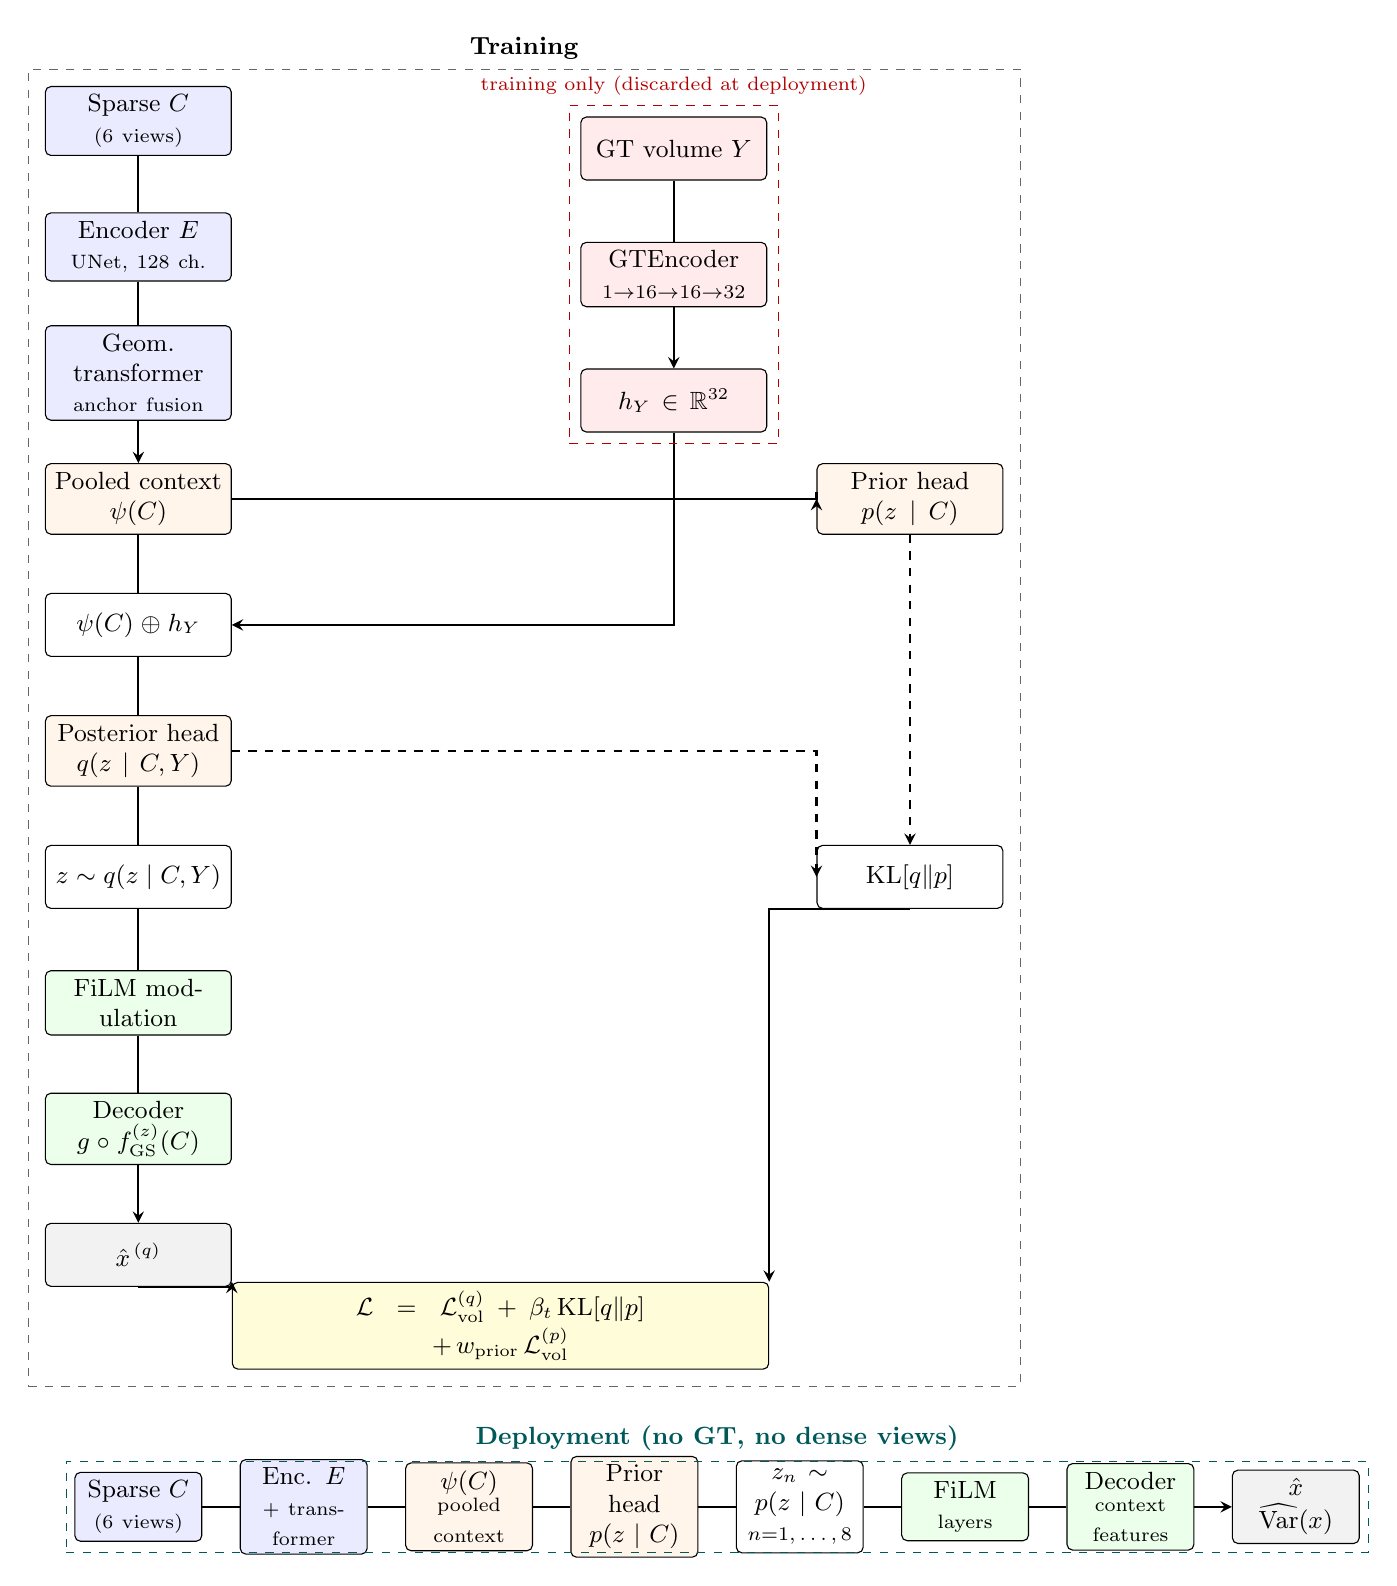
\begin{tikzpicture}[
    font=\small,
    >=stealth,
    box/.style={draw, rounded corners=2pt, align=center, inner sep=3pt,
                minimum height=8mm, text width=2.15cm},
    enc/.style={box, fill=blue!8},
    head/.style={box, fill=orange!8},
    gtenc/.style={box, fill=red!8},
    dec/.style={box, fill=green!8},
    outbox/.style={box, fill=gray!10},
    loss/.style={box, fill=yellow!15, text width=6.6cm},
    arr/.style={thick, ->},
    das/.style={thick, dashed, ->},
]
% ---- training column x=0, vertical spacing 1.6cm --------------------
\node[enc]   (C)    at (0, 0)       {Sparse $C$\\\scriptsize (6 views)};
\node[enc]   (E)    at (0, -1.6)    {Encoder $E$\\\scriptsize UNet, 128 ch.};
\node[enc]   (TF)   at (0, -3.2)    {Geom. transformer\\\scriptsize anchor fusion};
\node[head]  (PSI)  at (0, -4.8)    {Pooled context\\$\psi(C)$};
\node[box]   (CONC) at (0, -6.4)    {$\psi(C)\oplus h_Y$};
\node[head]  (Q)    at (0, -8.0)    {Posterior head\\$q(z\mid C,Y)$};
\node[box]   (ZQ)   at (0, -9.6)    {$z\sim q(z\mid C,Y)$};
\node[dec]   (FILM) at (0, -11.2)   {FiLM modulation};
\node[dec]   (DEC)  at (0, -12.8)   {Decoder\\$g\circ f_{\mathrm{GS}}^{(z)}(C)$};
\node[outbox](XQ)   at (0, -14.4)   {$\hat{x}^{\,(q)}$};
\node[loss]  (LOSS) at (4.6, -15.3) {$\mathcal{L}=\mathcal{L}_{\mathrm{vol}}^{(q)}
   +\beta_t\,\mathrm{KL}[q\|p]$\\[1pt]
   $+\,w_{\mathrm{prior}}\,\mathcal{L}_{\mathrm{vol}}^{(p)}$};

\node[gtenc] (Y)    at (6.8, -0.35) {GT volume $Y$};
\node[gtenc] (GTE)  at (6.8, -1.95) {GTEncoder\\\scriptsize $1{\to}16{\to}16{\to}32$};
\node[gtenc] (hY)   at (6.8, -3.55) {$h_Y\in\mathbb{R}^{32}$};
\node[head]  (PriH) at (9.8, -4.8)  {Prior head\\$p(z\mid C)$};
\node[box]   (KL)   at (9.8, -9.6)  {$\mathrm{KL}[q\|p]$};

\draw[arr] (C) -- (E) -- (TF) -- (PSI);
\draw[arr] (Y) -- (GTE) -- (hY);
\draw[arr] (hY.south) |- (CONC.east);
\draw[arr] (PSI) -- (CONC) -- (Q) -- (ZQ) -- (FILM) -- (DEC) -- (XQ);
\draw[arr] (PSI.east) -| (PriH.west);
\draw[arr] (XQ.south) -| (LOSS.north west);
\draw[das] (Q.east) -| (KL.west);
\draw[das] (PriH.south) -| (KL.north);
\draw[arr] (KL.south) -| (LOSS.north east);

\node[draw=red!70!black, dashed, fit=(Y)(GTE)(hY), inner sep=4pt,
      label={[red!70!black, font=\scriptsize]above:training only (discarded at deployment)}] {};
\node[draw=black!60, dashed, fit=(C)(LOSS)(KL)(Y), inner sep=6pt,
      label={[font=\small\bfseries]above:Training}] {};

% ---- deployment row y=-17.6, spacing 2.1cm --------------------------
\node[enc, text width=1.4cm]   (DC)    at (0.0, -17.6)  {Sparse $C$\\\scriptsize (6 views)};
\node[enc, text width=1.4cm]   (DE)    at (2.1, -17.6)  {Enc. $E$\\\scriptsize + transformer};
\node[head, text width=1.4cm]  (DPSI)  at (4.2, -17.6)  {$\psi(C)$\\\scriptsize pooled\\context};
\node[head, text width=1.4cm]  (DPRI)  at (6.3, -17.6)  {Prior head\\$p(z\mid C)$};
\node[box, text width=1.4cm]   (DZ)    at (8.4, -17.6)  {$z_n\sim p(z\mid C)$\\\scriptsize $n{=}1,\dots,8$};
\node[dec, text width=1.4cm]   (DFILM) at (10.5, -17.6) {FiLM\\\scriptsize layers};
\node[dec, text width=1.4cm]   (DDEC)  at (12.6, -17.6) {Decoder\\\scriptsize context\\features};
\node[outbox, text width=1.4cm](DX)    at (14.7, -17.6) {$\hat{x}$\\[1pt]$\widehat{\mathrm{Var}}(x)$};

\draw[arr] (DC) -- (DE) -- (DPSI) -- (DPRI) -- (DZ) -- (DFILM) -- (DDEC) -- (DX);

\node[draw=teal!70!black, dashed, fit=(DC)(DX), inner sep=3pt,
      label={[font=\small\bfseries, teal!70!black]above:Deployment (no GT, no dense views)}] {};
\end{tikzpicture}}
\end{figure}
%%
%% Chapter 4: Experiments
%% Independent file, included by ../main.tex
%%

\section{Experiments}
\label{sec:exp}

\subsection{Data and Protocol}
\label{sec:exp:protocol}

We evaluate on LUNA16 \cite{setio2017luna16} with the CBCT projection
simulator used in \cite{lin2024difgaussian}. The dataset is split into
738 training, 50 evaluation, and 100 test cases. Unless stated otherwise,
all models are trained from random initialization with the official
400-epoch protocol: 738 optimizer updates per epoch (batch size 1),
AdamW with $\mathrm{lr}=2{\times}10^{-4}$, per-epoch StepLR decay
$(10^{-3})^{1/400}$ per epoch, global gradient clipping at 1.0, FP32
precision, and a fixed random seed. The sparse context always consists
of the same six fixed projections with raw IDs $\{0,8,16,25,33,41\}$;
the dense training set contains 48 views. The network samples a random
sub-volume block and 1024 query points per step and is supervised in
volume space. Models are checkpointed every 20 epochs; the primary
comparison uses the final (epoch 400) model, and a supplementary
best-eval column reports the best PSNR over the 20 evaluation nodes.
Following the deterministic protocol, all probabilistic variants report
$N{=}8$ Monte-Carlo prior-mean estimates at inference. Metrics are peak
signal-to-noise ratio (PSNR, dB) and structural similarity (SSIM) on
the evaluation volumes at native scale.

\subsection{Implementation Details}
\label{sec:exp:impl}

All variants share the backbone of Section~\ref{sec:method:backbone}:
UNet encoder ($out\_ch=128$), geometry-transformer fusion with
parameters as in the released configuration (2 blocks, 4 heads, window
$\pm1$, feature scales $\{4,8,16\}$, $K{=}512$ anchors at resolution 12,
token initialization \texttt{max}). The probabilistic layer uses a
64-dimensional global latent; the FiLM modulation is initialized with
zero-mean weights of std $10^{-3}$ so that early training behaves like
the deterministic model. The GT encoder is a 3D CNN with channel
sizes $(1,16,16,32)$ and two stride-2 convolutions, followed by global
mean pooling, producing a 32-dimensional case descriptor. The posterior
head therefore receives a $128+7+32$-dimensional conditioning
vector. Prior and posterior heads share the bounded-Gaussian
parameterization with $\sigma\in[0.001,3.0]$ and
$\sigma_{\mathrm{init}}=0.5$. The KL is annealed linearly over 500 steps
to $\beta_f{=}2{\times}10^{-2}$ with a free-bits floor of $0.5$ nats;
the decoder conditions on the context set
(\texttt{posterior\_decoder\_views='context'}).

\subsection{Main Results}
\label{sec:exp:main}

Table~\ref{tab:results} reports reconstruction quality on the LUNA16
evaluation set. Several findings stand out.

\begin{table}[t]
\centering
\small
\setlength{\tabcolsep}{4pt}
\caption{Reconstruction quality on LUNA16 (six sparse views). Final
refers to the epoch-400 protocol model; best-eval reports the best PSNR
checkpoint over the 20 evaluation nodes. All probabilistic numbers use
the deployment-side estimator (prior MC mean, $N{=}8$), which never
touches dense views or ground truth.}
\label{tab:results}
\begin{tabular}{@{}p{3.3cm}p{2.5cm}ccc@{}}
\toprule
Model & Variant & PSNR (dB) & SSIM & Best-eval PSNR (dB) \\
\midrule
Deterministic backbone \cite{lin2024difgaussian} & -- & 29.54 & 0.870 & -- \\
\midrule
GT-CVAE & max-init, run~1 & 29.50 & 0.868 & 29.50 (E400) \\
GT-CVAE & max-init, run~2 & 29.06 & 0.854 & 29.06 (E400) \\
GT-CVAE & mean-init, run~1 & 27.55 & 0.808 & -- \\
GT-CVAE & mean-init, run~2 & 26.96 & 0.779 & -- \\
\bottomrule
\end{tabular}
\end{table}

\emph{The GT-conditioned CVAE reaches deterministic-level quality while
emitting uncertainty.}
The best GT-conditioned CVAE run reaches $29.50$\,dB / $0.868$\,SSIM at
the epoch-400 checkpoint, essentially matching the deterministic
backbone ($29.54$\,dB / $0.870$\,SSIM, a gap of only
$0.04$\,dB), while additionally emitting per-point predictive variance. Crucially, all of these numbers come from the
\emph{deployment} estimator ($z\sim p(z\mid C)$, no GT), so the reported
accuracy is what an operator would actually obtain.

\emph{The GT-conditioned posterior costs almost nothing.}
The model conditions its posterior on the ground-truth volume during
training, yet matches the deterministic backbone to within $0.04$\,dB
under the same \texttt{token\_init=max} setting. This confirms that
encoding the target into the variational posterior concentrates the
latent on case-specific content without overfitting the target, and
that the deployment-side prior retains the information needed for
accurate reconstruction.

\emph{Token initialization matters more than posterior design.} With
\texttt{token\_init\allowbreak=mean} both runs collapse to
$\approx 27$\,dB, a gap of roughly 2\,dB to the \texttt{max}-initialized
runs. All other settings are identical; the mechanism is analyzed in
Section~\ref{sec:exp:ablation}.

\subsection{Ablations}
\label{sec:exp:ablation}

\textbf{GT conditioning.}
Given the same \texttt{max} token initialization, the GT-conditioned
posterior (which encodes the ground truth during training) reaches
$29.06$--$29.50$\,dB against $29.54$\,dB for the deterministic
backbone, confirming that the GT-conditioned posterior provides the
intended information concentration without overfitting the target.

\textbf{Token initialization.}
Table~\ref{tab:results} shows a systematic effect:
\texttt{mean} \emph{vs.} \texttt{max} fusion of view tokens into
anchors changes the model's final PSNR by $\sim\!2$\,dB ($27.0$--$27.5$ vs.\
$29.1$--$29.5$\,dB). We attribute this to the interaction between token
initialization and the FiLM-gated latent: with \texttt{mean}
initialization the anchor features are more uniform, the fusion
transformer saturates earlier, and the latent has less discriminating
signal to modulate.
%%
%% Chapter 5: Conclusion
%% Independent file, included by ../main.tex
%%

\section{Conclusion}
\label{sec:conclusion}

We presented the GT-conditioned CVAE, a conditional variational
extension of Gaussian-splatting-based sparse-view CBCT reconstruction.
The model encodes the ground-truth volume into the variational posterior
$q(z\mid C,Y)$ during training through a lightweight 3D CNN, yet
discards both the GT encoder and the dense views at deployment,
sampling exclusively from a sparse-view neural-process prior
$p(z\mid C)$. On the LUNA16 benchmark with six projections, the model
reaches $29.50$\,dB PSNR / $0.868$\,SSIM (best-eval), within $0.04$\,dB
of the deterministic backbone, while providing per-point predictive
variance at no additional inference cost.

The central methodological insight of this paper is that two design
choices carry the method. First, the decoder is conditioned on the
sparse context features, so the latent is the \emph{sole} channel
through which dense information reaches the volume during training;
this keeps the latent informative without any train/deploy mismatch.
Second, ablations show that \texttt{max}-fused anchor tokens preserve
the latent's discriminating signal, worth roughly $2$\,dB over
\texttt{mean} initialization. With these choices, the GT-conditioned
posterior concentrates the latent on case-specific content during
training at no cost at deployment.

\textbf{Future work} includes (i) validating the GT-conditioned design
under additional context counts and denser view schedules,
(ii) extending the model to hierarchical local latents for fine-grained
uncertainty maps, (iii) calibrating the predictive variance against
real reconstruction errors for use in dose-guided adaptive
radiotherapy, and (iv) transferring the information-flow design to other
modality-paired inverse problems (e.g., sparse-view MRI, low-dose PET).

\section*{Acknowledgements}

The authors gratefully acknowledge the computing resources and the
LUNA16 challenge data \cite{setio2017luna16}. The authors declare no
conflict of interest.

%% References ------------------------------------------------
\section*{References}
\bibliographystyle{elsarticle-num}
\bibliography{refs}

%% Key code snippets (GT encoder, posterior path, released config)
\appendix
%%
%% Appendix: Key code snippets
%% Independent file, included by ../main.tex
%%

\section{Key Code Snippets}
\label{app:code}

We provide the three most relevant fragments of the released
implementation for reproducibility: the lightweight GT encoder
(Listing~\ref{lst:gt_encoder}), the conditional posterior path inside
the probabilistic model (Listing~\ref{lst:posterior}), and the released
configuration used for the reported results
(Listing~\ref{lst:config}).

\subsection{GT Encoder}
\label{app:code:gt}

The GT encoder is a lightweight 3D CNN that maps the ground-truth volume
to a feature volume and mean-pools it into a 32-dimensional global
descriptor $h_Y$. It is instantiated only in \texttt{gt\_cvae} mode and
only consumed during training.

\begin{lstlisting}[language=Python, caption={models/gt\_encoder.py: the
GT encoder.}, label={lst:gt_encoder}]
class GTEncoder(nn.Module):
    """Maps a GT CT volume to a feature volume, then pools a global
    feature for the variational posterior."""

    def __init__(self, in_ch=1, out_ch=32, mid_ch=16):
        super().__init__()
        self.out_ch = out_ch
        self.net = nn.Sequential(
            nn.Conv3d(in_ch, mid_ch, kernel_size=3, padding=1),
            nn.GroupNorm(4, mid_ch),
            nn.SiLU(inplace=True),
            nn.Conv3d(mid_ch, mid_ch, kernel_size=3, stride=2, padding=1),
            nn.GroupNorm(4, mid_ch),
            nn.SiLU(inplace=True),
            nn.Conv3d(mid_ch, out_ch, kernel_size=3, stride=2, padding=1),
            nn.GroupNorm(4, out_ch),
            nn.SiLU(inplace=True),
        )

    def forward(self, gt_volume, anchor_xyz=None):
        """gt_volume: [B, 1, D, H, W]  ->  feat_volume + gt_global_feat."""
        if gt_volume.dim() == 4:
            gt_volume = gt_volume.unsqueeze(1)
        feat_volume = self.net(gt_volume)
        gt_global_feat = feat_volume.mean(dim=(2, 3, 4))   # [B, 32]
        return {'feat_volume': feat_volume,
                'gt_global_feat': gt_global_feat}
\end{lstlisting}

\subsection{Conditional Posterior Path}
\label{app:code:posterior}

During training the sparse context is encoded once into the pooled
representation $\psi(C)$; in \texttt{gt\_cvae} mode the posterior head
instead receives $\psi(C)\oplus h_Y$ computed from the ground-truth
volume. The decoder always renders from \emph{context} features (the
released \texttt{posterior\_decoder\_views='context'}), so the FiLM
modulated latent is the only privileged channel.

\begin{lstlisting}[language=Python, caption={models/dense\_probability.py:
context encoding (top) and the conditional posterior path (middle), with
FiLM modulation of the decoder features (bottom).},
label={lst:posterior}]
def encode_context(self, data, prepare=True):
    clean = context_inputs(data)
    if prepare:
        clean = self.prepare_views(clean)
    features = self.encode_projs(clean)
    pooled = torch.cat([features['anchor_feats'].mean(-1),
                        observation_descriptor(clean)], -1)
    return ContextState(features, clean, pooled, grid=None)

def infer_posterior(self, data, context, dense=None):
    """GT-conditioned CVAE (gt_cvae): condition q(z | C, Y) on the GT
    volume, not on dense views. GT encoder is never called when
    gt_volume is None."""
    if self.mode == 'dense_np':
        dense = dense if dense is not None else self.encode_dense(data)
        pooled, grid = dense.pooled, dense.grid     # 48 dense views
    else:
        if data.get('gt_volume') is None:
            raise ValueError('gt_cvae posterior requires gt_volume')
        gt = self.gt_encoder(data['gt_volume'],
                             context.data['points_gs'])
        pooled = torch.cat([context.pooled,
                            gt['gt_global_feat']], -1)   # 128+7+32
        grid = None                                     # use_local=False
    return self.posterior_head(pooled), grid

# in sample_state(): draw z and modulate the *context* features
mu, lv = posterior if posterior is not None else prior
z_g = mu if mean else reparameterize(mu, lv, generator)
features['gs_params']['feats'] = self.feature_film(
    context.features['gs_params']['feats'], z_g)
\end{lstlisting}

\subsection{Released Configuration}
\label{app:code:config}

The released configuration (which produced the results reported in
Section~\ref{sec:exp}) fixes the mode to \texttt{gt\_cvae}, uses a
64-dimensional global latent with no local latent
(\texttt{use\_local: false}), a per-dimension free-bits floor of
$0.5$ nats, an annealed $\beta_f=2{\times}10^{-2}$, and the
\emph{prior mean} Monte-Carlo estimator with $N{=}8$ samples at
inference.

\begin{lstlisting}[caption={configs/experiment\_plan/stage1/
prob-gt-cvae.yaml (excerpt): the released model, objective and
evaluation blocks. \texttt{posterior\_decoder\_views} is not a config
key; the code default is \texttt{'context'}.},
label={lst:config}]
model:
  image_encoder:
    out_ch: 128
  anchor_fusion: geometry_transformer
  point_fusion: max
  multiview_transformer:
    d_model: 128
    num_heads: 4
    num_blocks: 2
    feature_scales: [4, 8, 16]
    samples_per_scale: 5
    spatial_window: 3        # window of +-1 anchor neighbors
    token_init: max          # max-fused anchor tokens (ablation: mean)
  gs:
    t: 512
    res: 12
  probabilistic:
    mode: gt_cvae            # GT-conditioned CVAE posterior
    objective: joint
    normalization: groupnorm_anchor_instance
    film_init_std: 1.0e-3    # zero-mean FiLM init (deterministic start)
    train_samples: 1
    latent:
      global_dim: 64         # z in R^64, FiLM-injected
      use_local: false       # global latent only
      sigma_min: 0.001
      sigma_max: 3.0
      initial_sigma: 0.5
    reconstruction:
      likelihood: mse
      observation_sigma: 0.1   # sigma_obs for the Gaussian likelihood
      reduction: mean_query
    kl:
      beta_final: 2.0e-02      # annealed over warmup
      warmup_steps: 500
      free_bits: 0.5           # per-dimension KL floor (nats)
      free_bits_order: per_case
      reduction: sum_latent_mean_batch
    evaluation:
      estimator: prior_mc_mean  # z ~ p(z|C), mean over samples
      num_samples: 8
dataset:
  paired_views:
    dense_count: 48             # training-only side information
    context_counts: [6]         # deployment view budget
\end{lstlisting}

\end{document}